\begin{center}

\includegraphics[width=0.4\textwidth]{content/3/chapter7/images/18.png}\\
Cippi挖花园的地
\end{center}

在修改co\_await章节的工作流之前,我想让待等待的工作流更加透明。


\subsubsubsection{7.4.1\hspace{0.2cm}透明的待等待的工作流}

我在startJob.cpp中添加了一些输出。

\begin{lstlisting}[style=styleCXX]
// startJobWithComments.cpp

#include <coroutine>
#include <iostream>

struct MySuspendAlways {
	bool await_ready() const noexcept {
		std::cout << " MySuspendAlways::await_ready" << '\n';
		return false;
	}
	void await_suspend(std::coroutine_handle<>) const noexcept {
		std::cout << " MySuspendAlways::await_suspend" << '\n';
	
	}
	void await_resume() const noexcept {
		std::cout << " MySuspendAlways::await_resume" << '\n';
	}
};

struct MySuspendNever {
	bool await_ready() const noexcept {
		std::cout << " MySuspendNever::await_ready" << '\n';
		return true;
	}
	void await_suspend(std::coroutine_handle<>) const noexcept {
		std::cout << " MySuspendNever::await_suspend" << '\n';
	
	}
	void await_resume() const noexcept {
		std::cout << " MySuspendNever::await_resume" << '\n';
	}
};
	
struct Job {
	struct promise_type;
	using handle_type = std::coroutine_handle<promise_type>;
	handle_type coro;
	Job(handle_type h): coro(h){}
	~Job() {
		if ( coro ) coro.destroy();
	}
	void start() {
		coro.resume();
	}
	
	
	struct promise_type {
		auto get_return_object() {
			return Job{handle_type::from_promise(*this)};
		}
		MySuspendAlways initial_suspend() {
			std::cout << " Job prepared" << '\n';
			return {};
		}
		MySuspendAlways final_suspend() noexcept {
			std::cout << " Job finished" << '\n';
			return {};
		}
		void return_void() {}
		void unhandled_exception() {}
	
	};
};

Job prepareJob() {
	co_await MySuspendNever();
}

int main() {

	std::cout << "Before job" << '\n';
	
	auto job = prepareJob();
	job.start();
	
	std::cout << "After job" << '\n';

}
\end{lstlisting}

首先,我用可等待对象MySuspendAlways(第6行)和MySuspendNever(第20行)替换了预定义的可等待对象std::suspend\_always和std::suspend\_never,在第51、55和66行使用了它们。这些可等待对象模仿预定义的可等待对象的行为,但还要加点注解。由于使用std::cout,所以成员函数await\_ready、await\_suspend和await\_resume不能声明为constexpr。

程序执行的屏幕截图很好地显示了控制流,可以直接在\href{https://godbolt.org/z/T5rcE4}{Compiler Explorer}上观察到。

\begin{center}
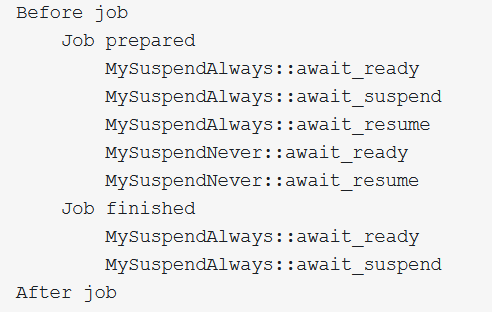
\includegraphics[width=0.8\textwidth]{content/3/chapter7/images/19.png}\\
根据请求开启工作(包括注解)
\end{center}

函数initial\_suspend(第51行)在协程的开头执行,final\_suspend在协程的末尾执行(第55行)。prepareJob()(第73行)触发了协程对象的创建,函数调用job.start()恢复了协程对象,因此完成了协程对象的创建(第74行)。因此,MySuspendAlways的await\_ready、await\_suspend和await\_resume成员将执行。在不恢复成员函数final\_suspend返回的可等待对象(例如:协程对象)的情况下,不会处理await\_resume。相反,MySuspendNever函数是立即执行的,因为await\_ready返回true,所以不会挂起。通过这些注解,读者们应该对待等待的工作流有了基本的了解。

现在,来改变它吧。

\subsubsubsection{7.4.2\hspace{0.2cm}自动恢复的Awaiter}

前面的工作流中,我显式地启动了该任务。

\begin{lstlisting}[style=styleCXX]
int main() {
	
	std::cout << "Before job" << '\n';
	
	auto job = prepareJob();
	job.start();
	
	std::cout << "After job" << '\n';
	
}
\end{lstlisting}

显式调用job.start()是必要的,因为MySuspendAlways中的await\_ready总是返回false。现在假设await\_ready可以返回true或false,并且任务没有显式地启动。一个简短的提醒:当await\_ready返回true时,函数await\_resume(不是await\_suspend)会直接调用。

\begin{lstlisting}[style=styleCXX]
// startJobWithAutomaticResumption.cpp

#include <coroutine>
#include <functional>
#include <iostream>
#include <random>

std::random_device seed;
auto gen = std::bind_front(std::uniform_int_distribution<>(0,1),
						   std::default_random_engine(seed()));

struct MySuspendAlways {
	bool await_ready() const noexcept {
		std::cout << " MySuspendAlways::await_ready" << '\n';
		return gen();
	}
	bool await_suspend(std::coroutine_handle<> handle) const noexcept {
		std::cout << " MySuspendAlways::await_suspend" << '\n';
		handle.resume();
		return true;
	
	}
	void await_resume() const noexcept {
		std::cout << " MySuspendAlways::await_resume" << '\n';
	}
};

struct Job {
	struct promise_type;
	using handle_type = std::coroutine_handle<promise_type>;
	handle_type coro;
	Job(handle_type h): coro(h){}
	~Job() {
		if ( coro ) coro.destroy();
	}
	
	struct promise_type {
		auto get_return_object() {
			return Job{handle_type::from_promise(*this)};
		}
		MySuspendAlways initial_suspend() {
		std::cout << " Job prepared" << '\n';
			return {};
		}
		std::suspend_always final_suspend() noexcept {
			std::cout << " Job finished" << '\n';
			return {};
		}
		void return_void() {}
		void unhandled_exception() {}
	
	};
};

Job performJob() {
	co_await std::suspend_never();
}

int main() {

	std::cout << "Before jobs" << '\n';
	
	performJob();
	performJob();
	performJob();
	performJob();
	
	std::cout << "After jobs" << '\n';

}
\end{lstlisting}

首先,协程现在称为performJob并自动运行。gen(第9行)是数字0或1的随机数生成器,其使用默认的随机引擎,用种子初始化。因为std::bind\_front,所以可以将它与std::uniform\_int\_distribution绑定在一起,以获得一个可调用对象。在使用时,会生成出一个随机数0或1。

这个例子中,我从C++标准中删除了带有预定义可等待对象的可等待对象,除了作为成员函数initial\_suspend返回类型的可等待对象MySuspendAlways(第41行)。await\_ready(第13行)返回一个布尔值。当布尔值为true时,控制流直接跳转到成员函数await\_resume(第23行);当为false时,协程立即挂起。因此,函数await\_suspend运行(第17行)。函数await\_suspend获取协程句柄,并使用它来恢复协程(第19行)。而不是返回值true, await\_suspend也可以返回void。

下面的截图显示:当await\_ready返回true时,调用await\_resume函数,当await\_ready返回false时,调用await\_suspend函数。

读者们可以在\href{https://godbolt.org/z/8b1Y14}{Compiler Explorer}上尝试编译和运行该程序。

\begin{center}
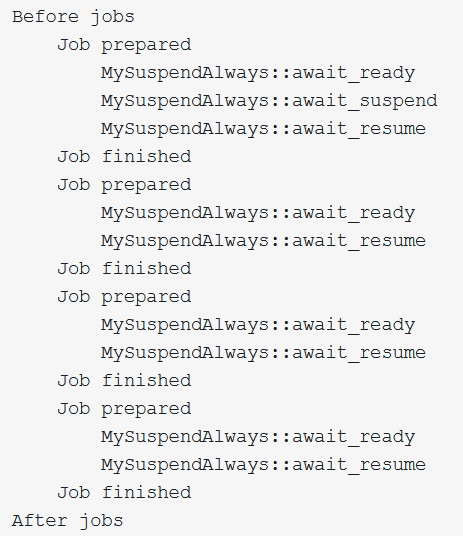
\includegraphics[width=0.8\textwidth]{content/3/chapter7/images/20.png}\\
自动恢复的Awaiter
\end{center}

让我进一步改进程序,并在单独的线程上恢复待等待对象。

\subsubsubsection{7.4.3\hspace{0.2cm}自动恢复单独线程上的Awaiter}

下面的程序是在前一个程序的基础上编写的。

\hspace*{\fill} \\ %插入空行
\noindent
\textbf{一个单独的线程上自动恢复Awaiter}
\begin{lstlisting}[style=styleCXX]
// startJobWithAutomaticResumptionOnThread.cpp

#include <coroutine>
#include <functional>
#include <iostream>
#include <random>
#include <thread>
#include <vector>

std::random_device seed;
auto gen = std::bind_front(std::uniform_int_distribution<>(0,1),
						   std::default_random_engine(seed()));

struct MyAwaitable {
	std::jthread& outerThread;
	bool await_ready() const noexcept {
		auto res = gen();
		if (res) std::cout << " (executed)" << '\n';
		else std::cout << " (suspended)" << '\n';
		return res;
	}
	void await_suspend(std::coroutine_handle<> h) {
		outerThread = std::jthread([h] { h.resume(); });
	}
	void await_resume() {}
};


struct Job{
	static inline int JobCounter{1};
	Job() {
		++JobCounter;
	}

	struct promise_type {
		int JobNumber{JobCounter};
		Job get_return_object() { return {}; }
		std::suspend_never initial_suspend() {
			std::cout << " Job " << JobNumber << " prepared on thread "
			          << std::this_thread::get_id();
			return {};
		}
		std::suspend_never final_suspend() noexcept {
			std::cout << " Job " << JobNumber << " finished on thread "
			          << std::this_thread::get_id() << '\n';
			return {};
		}
		void return_void() {}
		void unhandled_exception() { }
	};
};

Job performJob(std::jthread& out) {
	co_await MyAwaitable{out};
}

int main() {

	std::vector<std::jthread> threads(8);
	for (auto& thr: threads) performJob(thr);

}
\end{lstlisting}

与前一个程序的区别在于,协程performJob中使用了新的可等待MyAwaitable(第54行)。相反,从协程performJob返回的协程对象很简单,它的成员函数initial\_suspend(第38行)和final\_suspend(第43行)返回预定义的可等待std::suspend\_never。此外,这两个函数都显示所执行作业的JobNumber和所运行的线程ID。屏幕截图显示了哪个协程立即运行,哪个挂起。多亏了线程id,才可以观察到挂起的协程在另一个线程上恢复了。

读者们可以在\href{https://wandbox.org/permlink/skHgWKF0SYAwp8Dm}{Wandbox}上尝试该程序。

\begin{center}
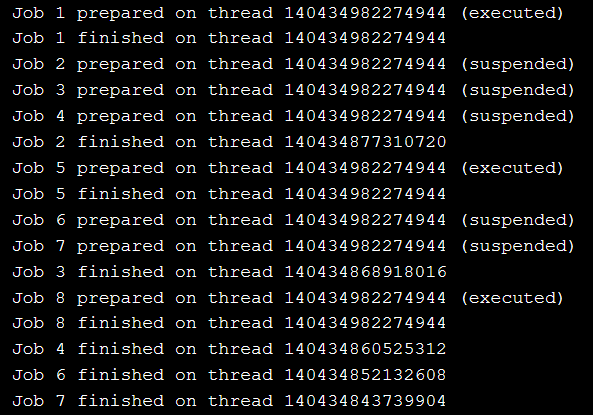
\includegraphics[width=0.8\textwidth]{content/3/chapter7/images/21.png}\\
自动恢复单独线程上的Awaiter
\end{center}

来讨论一下这个程序的有趣的控制流程。第59行创建了8个默认构造的线程,协程performJob(第53行)通过引用接受这些线程。此外,引用成为创建MyAwaitable\{out\}的参数(第54行)。根据res的值(第17行),以及函数await\_ready的返回值,协程将继续(res为true)运行或挂起(res为false)。若MyAwaitable挂起,函数await\_suspend(第22行)将执行。由于分配了outerThread(第23行),其变成了一个正在运行的线程,从而生命周期必须比协程的长。因此,线程具有main函数的作用域。

\begin{tcolorbox}[breakable,enhanced jigsaw,colback=mygreen!5!white,colframe=mygreen!75!black,title={总结}]
	
\begin{itemize}
\item 
想要多次同步线程时,有许多选项。可以使用条件变量、std::atomic\_flag、std::atomic<bool>或信号量。这个案例研究回答了一个问题:哪个变体是最快的?数字表明,条件变量是最慢的方式,原子标记是同步线程的最快方式。std::atomic<bool>的性能介于两者之间,信号量几乎和原子标志一样快。

\item 
使用co\_return,协程的章节中介绍了一个立即执行的future。这个future是一个理想的起点,可以让它变得懒惰,最后让它在自己的线程上运行。

\item 
对无限数据流的生成器的修改了解了其本质。当成员函数initial\_suspend返回std::suspend\_never时,协程立即启动并忽略第一个值。相反,从函数yield\_value返回std::suspend\_never将以无限循环结束。当忘记恢复协程时,其将永远不会运行。

\item 
泛型Generator<T>,可以连续返回标准模板库中任意容器的元素,而不是无限的数据流。

\item 
实现自己的可等待的MySuspendNever和MySuspendAlways使等待工作流透明。调整可等待的MySuspendAlways使其能够创建一个在必要时恢复自身的Awaiter。

\item 
修改可等待对象,可使协程在其他线程上恢复运行。
\end{itemize}
	
\end{tcolorbox}




















